\documentclass[12pt,addpoints,answers]{exam}
\usepackage{mystyle}
\usepackage[margin=0.4cm, landscape, b4paper]{geometry}

\begin{document}
\bracketedpoints
\pagestyle{headandfoot}
\mylogo
\begin{questions}
\question From a group of 5 assistant professors, 6 associate professors, and 4 professors, a group of 2 assistant professors, 2 associate professors, and 3 professors need to be chosen to form a thesis committee of 7 members;  How many different such thesis committees are possible?
\question 9 computers are brought in for servicing (and machines are serviced one at a time). Of the 9 computers, 3 are PCs, 4 are Macs, and 2 are Linux machines. Assume that all computers of the same type are indistinguishable (i.e., all the PCs are indistinguishable, all the Macs are indistinguishable, etc.).
\begin{parts}
\part In how many distinguishable ways can the computers be ordered for servicing?
\part In how many distinguishable ways can the computers be ordered if the first 5 machines serviced must include all 4 Macs?
\part In how many distinguishable ways can the computers be ordered if 2 PCs must be in the first three and 1 PC must be in the last three computers serviced?
\end{parts}
\question Say you have 20 lakh rupees that must be invested among 4 possible companies. Each investment must be in integral units of
1 lakh rupees, and there are minimal investments that need to be made if one is to invest in these companies. The minimal investments are 1, 2, 3, and 4 lakh rupees, respectively for company 1, 2, 3, and 4. How many different investment strategies are available if:
\begin{parts}
\part an investment must be made in each company?
\part investments must be made in at least 3 of the 4 companies?
\end{parts}
\question Eleven soccer players are to be divided into $4$ functional groups: $3$ forwards, $3$ midfields, $4$ defenses, and $1$ goalie. There are only $2$ people who can play goalie. Both of these two players can play any other position. Of the remaining $9$, $4$ can play only forward or midfield; the other $5$ can play only defense or midfield. We want to calculate the number of possible ways to divide the team into the $4$ functional groups. Follow the hint below and get to the answer:
\begin{align*}
\text{Select 1 goalie out of 2 in } \binom{?}{?}\text{ ways \textbf{\color{red}AND}} &\begin{cases}\text{Remaining goalie plays defense}\\\qquad\qquad\qquad\textbf{\color{blue}OR}\\\text{Remaining goalie plays midfield}\\\qquad\qquad\qquad\textbf{\color{blue}OR}\\\text{Remaining goalie plays forward}\end{cases}
\end{align*}
\question In how many ways can $r$ identical server requests be distributed among $n$ servers so that the $i$th server receives \emph{at least} $m_i$ requests, for each $i = 1,2,\ldots,n$? You can assume that $r \geq (m_1+m_2+\cdots+m_n).$
\question Suppose a particle starting from the origin can move \emph{only} up or down; the \emph{binomial option pricing model} addresses stock price movements using such an idea. 
\begin{center}
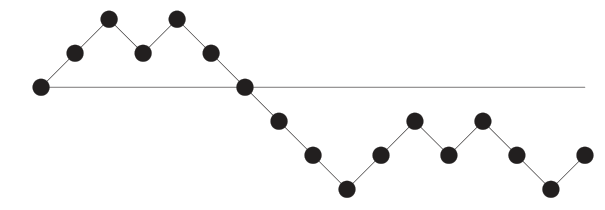
\includegraphics[keepaspectratio, scale = 0.7]{binomialmove.png}
\end{center}
Show that the number of ways the particle can move from the origin to position $k$ in $n$ steps is $\binom{n}{\frac{n+k}{2}}.$ Assume that $n+k$ is even.
\end{questions}
\label{totalpag}
\end{document}


 